\documentclass{scrartcl}
\usepackage[utf8]{inputenc}
\usepackage[T1]{fontenc}
\usepackage[ngerman]{babel}
\usepackage{amsmath}
\usepackage{graphicx}
 
\title{Praktikum Betriebssysteme: Projekt 1\\ Client/Server Stream Socket Programmierung}
\author{Andreas Ruscheinski\thanks{Matr.-nr.: 211203494}\and Christian Delfs\thanks{Matr.-nr.: 211204103}\and Fabienne Lambusch\thanks{Matr.-nr.: ?????????}}
\begin{document}
\maketitle
\tableofcontents
\newpage
\section{Problem}
	Ziel des Projektes war es, zu lernen, wie Dateien mit Hilfe von Client/Server Stream Socket Programmierung (mit TCP/IP Sockets) angelegt und verwaltet werden können. Das wie folgt beschriebene Grundsystem wurde von uns mit einem Datei-Zugriffsschutz erweitert. 
	Unsere Gruppe hat sich für Option b) entschieden: den Datei-Zugriffsschutz. Hierbei wird zwischen normalen Nutzern und Administratoren unterschieden, die sich durch verschiedene Rechte auszeichnen. Nach einem Login, der zum einen die Gültigkeit prüft, werden an dieser Stelle auch die Rechte ermittelt. Durch die Rechteverteilung werden dem Nutzer auf Clientseite verschiedene Funktionen zur Auswahl gestellt.\\

\section{Vorbetrachtung - Theorie}
	\subsection{Grundfunktionalitäten}
		Die grundlegenden Anforderungen an das Softwarprojekt sind wie folgt gegeben:
		\begin{enumerate}
		\item Speicherung der Studenten in separate Datensätze auf der Server-Seite. Enthaltene Informationen: Name, Matrikel-Nr., Geburtsdatum, Noten von n
		Lehrveranstaltungen.
		\item Es gibt m Gruppen von Studenten, die jeweils mehrere Studenten umfassen (m >= 3).
		\item Jede Gruppe repräsentiert einen Studiengang.
		\item Die Datensätze jeder Gruppe werden in einer eigenen Datei gespeichert.
		\item Gruppenbesten anhand des Durchschnitts ermitteln.
		\item Mindestanforderungen: Mindestens drei Gruppen und in jeder: mindestens drei Studenten und jeder Studentendatei: mindestens drei Noten
		\item Die Datensätze der Studenten sollten zugreifbar sein.
		\item Bester aller Studenten soll ermittelbar sein.
		
		\end{enumerate}
	\subsection{Kommunikation zwischen Server und Client}
		
	\subsection{Dateizugriff}
		In unserm Projekt nutzen wir das CDV-Dateiformat um die Datensätze von Studenten auf eine praktische Art und Weise speichern und auslesen zu können. Um die Studenten ihrer zugehörigen Gruppen zuzuordnen, werden diese in Verzeichnissen abgelegt.\\
		Diese Verzeichnisse werden anhand ihrer Bennenungen unterschieden, z.B.: steht der Ordner ITTI für die Studenten, die der Informationstechnik / Technische Informatik angehören.\\
		Generell werden Studenten in einer Datei gespeichert, die als Bezeichnung die zughörige Matrikelnummer besitzt. Innerhalb der Datei befinden sich die folgenden Datensätze, durch Simikolons von einander getrennt:\\
		\begin{itemize}
			\item Passwort
			\item Vorname
			\item Nachname
			\item Matrikelnummer
			\item zugehöriger Studiengang
			\item Geburtstag
			\item eine beliebiege Anzahl an Noten
		\end{itemize}
		Der Datensatz eines Beispielstudenten sieht folgender Maßen aus:\\
		 \\
		mukitkarP;Max;Mustermann;113116119;Informatik;23.05.2013;1.0;1.3;2.7;5.0;1.0\\
		 \\
		Innerhalb des Programmes werden, bis auf die Noten, die Datensätze als Char-Arrays gespeichert. Wichtig ist es darauf zu achten, dass an letzter Stelle das Terminationszeichen ist. Das Passwort darf aus maximal 10 Zeichen bestehen. Für Vorname, Nachname und der zugehörige Studiengang sind 20+1 Char zur Verwendung unterstützt. Die Matrikelnummer besitzt 9 Stellen. Diese wird folglich in 9+1 Chars vom Client abgefragt. Ähnlich bei dem Geburtstag der in der Form DD.MM.YYYY in 11 Chars gespeichert wird. \\
		Sowohl die einzelnen Noten, als auch die berechneten Durschnitte sind vom Datentyp Double. In die Datei werden die Noten als Chars der Länge 4 eingetragen, sodass sie immer die folgende Form besitzen X.Y wobei 1<X<5 und Y$\in \{$0,3,7$\}$ ist.\\
		\subsubsection{Beipieldatein}
			Da zu Laufzeiten des Programms sowohl Gruppen als auch Studenten mit einer beliebigen Anzahl an Noten hinzugefügt werden, decken unsere Beispieldatein den geforderten Teil ab:\\
			\textbf{Gruppen:}
			\begin{itemize}
				\item Informatik
				\item ITTI
				\item Elektrotechnik
			\end{itemize}
			
			\textbf{Studenten der Informatik:}
			\begin{itemize}
				\item 123;Tom;Klein;?????????;Informatik;01.01.19901.0;4.0;1.7;3.0
				\item 234;Max;Mustermann;?????????;Informatik;23.05.2001;1.0;1.3;2.7
				\item 345;Benjamin;Groß;?????????;Informatik;14.12.1986;1.0;1.3;2.7;3.3;1.7;5.0
			\end{itemize}
			
			\textbf{Studenten der ITTI:}
			\begin{itemize}
				\item 456;Even;Longer;?????????;ITTI;15.11.1977;1.3;2.7;3.3;1.7;5.0;1.0
				\item 567;Very;Long;?????????;ITTI;12.05.1993;1.0;1.3;2.7;1.0;5.0;1.0;1.0;1.0
				\item 678;Alfons;Hatler;?????????;ITTI;14.03.1989;1.0;1.0;1.0;1.0
			\end{itemize}
			
			\textbf{Studenten der Elektrotechnik:}
			\begin{itemize}
				\item 789;John;McClane;?????????;Elektrotechnik;24.12.1966;1.3;3.7;5.0;4.0
				\item 890;Hans;Gruber;?????????;Elektrotechnik;15.07.1991;1.3;5.0;2.7;1.0;4.0;1.7;3.0;2.0
				\item 901;Holly;McClane;?????????;Elektrotechnik;30.08.1988;1.7;1.3;1.3;1.7;1.0;1.7;1.7
			\end{itemize}
		
	\subsection{Umzusetztende Funktionalitäten}
		Neben den geforderten Funktionen, haben wir unser Programm um einige ausgewählte Funktionen bereichert. Unter Berücksichtigung der zwei Zugriffsarten mit unterschiedlichen Rechten werden hier die Funktionalitäten an zugehöriger Stelle beschrieben.\\
		Dem Nutzer werden diese Möglichkeiten nach dem Login in einer Menüform zur Auswahl gestellt. Die Auswahl eines Menüpunktes erfragt auf Client-Seite, wenn nötig, Eingaben bzw. gibt die gewünschten Ergebnisse zurück.
		\subsubsection{Administrator}
			\begin{description}
				\item[Studenten anlegen] Der Administrator muss bei dem Erstellen eines neuen Studenten dessen Vorname, Nachname, Matrikelnummer, Studiengang und Geburtstag angeben. Durch diese Eingabe wird eine Datei mit der Matrikelnummer als Name und im passenden Ordner (dem Studiengang) angelegt.
				\item[Gruppe anlegen] Durch diese Funktion wird ein neues Verzeichnis erstellt, in das später Studenten eingefügt werden können.
				\item[Studentendaten anzeigen] Um die Daten eines Studenten einzusehen, werden Kentniss über seinen Studiengang und sine Matrikelnummer vorrausgesetzt. Zusätzlich wird auch dessen Durschnitt angezeigt.
				\item[Guppe anzeigen] Nach der Eingabe des Studiengangs als Gruppennamen, werden alle Studenten aus diesem ausgegeben.
				\item[Note hinzufügen] Damit einem Studenten eine Note hinzugefügt werden kann müssen Studiengang, Matrikelnummer und die hinzuzufügende Note als Eingabe angegeben werden.
				\item[Gruppenbesten ermitteln] Für die ausgewählte Gruppe wird der beste Student anhand der einzelnen Durchschnitte ermittelt.
				\item[Gesamtbesten ermitteln] Von allen Studenten, die gespeichert sind, wird der, mit dem besten Durchschnitt, ausgegeben.
				\item[Beenden] Beendet die Kommunikation mit dem Server und schließt das Programm auf Seite des Clients.
			\end{description}
			\subsubsection{Normale Nutzer}
			\begin{description}
				\item[Daten anzeigen] Neben dem  Vornamen, Nachnamen, Studiengang, Geburtstag und der Matrikelnummer wird der Durchschnitt ausgegeben.
				\item[Beenden] Beendet die Kommunikation mit dem Server und schließt das Programm auf Seite des Clients.
			\end{description}
\section{Praktische Umsetzung}
\subsection{Client}
\subsubsection{Menü}
	Die in Kapitel 2.4 Beschriebenen Funktionalitäten führen zu zwei unterschiedlichen Menü-Formen. Abhängig von den Rechten, die dem Nutzer nach dem Login zugeteilt werden, wird ein entsprechendes Menü angezeigt.
	
	\begin{center}
	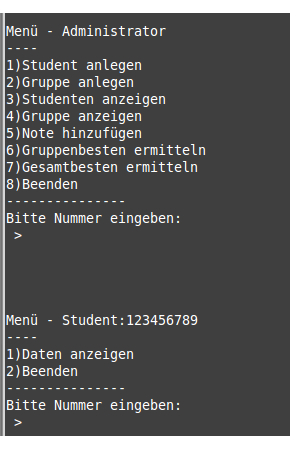
\includegraphics[scale=0.6]{menue.jpg}
	\end{center}
\subsubsection{Funktionen}
\subsubsection{Ausgaben}
\subsubsection{Menüführung}
\subsection{Server}
\subsubsection{Arbeitsweise}
\subsubsection{Funktionen}
\subsubsection{Ausgaben}
\section{Nutzerhandbuch}

\end{document}